\documentclass{article}
\usepackage[utf8]{inputenc}
\usepackage[T1]{fontenc}
\usepackage[margin=1in]{geometry}
\usepackage{graphicx}
\graphicspath{{figures/}}
\usepackage{booktabs}
\usepackage{longtable}
\usepackage{hyperref}
\usepackage{amsmath}
\usepackage[backend=biber,style=apa,sorting=ynt]{biblatex}
\addbibresource{references.bib}

\title{What Do We Actually Do With Our Voices?\\
A Two-Stage Study of Extreme Metal Vocal Practice}
\author{Alexey Voronin \and Nat Condit-Schultz}
\date{}

\begin{document}
\maketitle

\begin{abstract}
\textbf{Objectives:} Extreme metal voice research has made substantial progress in physiology and perception, but performer-centered descriptions of technique, training, and practical categorization remain underrepresented. We analyze how vocalists describe their own practice and whether a three-class perceptual scaffold (scream-like, growl-like, hybrid/shout-like) is usable from the performer perspective.\\
\textbf{Methods:} We used a two-stage design. Stage 1 consisted of 18 semi-structured one-on-one interviews coded into thematic segments (810 segments total). Stage 2 used a Qualtrics survey (72 total rows; 39 finished) and included both open-text prompts and a dedicated perceptual-class block (Q43--Q46). Partial responses were retained when they contained meaningful textual content.\\
\textbf{Results:} Stage 1 showed stable high-frequency thematic domains in musical background, taste/influence, perception/intelligibility, and technique/health narratives. In Stage 2, most respondents endorsed the three-class framework (Q43: 66.7\% agree), while technique-to-class mapping (Q44, \(N=38\)) showed both expected trends (low-register and guttural toward growl-like; high fry and banshee toward scream-like) and systematic overlap in mid/bridging techniques. Q46 indicated that explicit class-language is used inconsistently in everyday practice (20.0\% regularly, 47.5\% sometimes, 32.5\% rarely/never).\\
\textbf{Conclusions:} A two-stage mixed qualitative design supports a practically useful but gradient performer-centered taxonomy. Perceptual classes are interpretable for most vocalists, yet production terminology remains primary in day-to-day vocal reasoning.
\end{abstract}

\section{Introduction}
Extreme metal vocalization is frequently described through two partially overlapping vocabularies. The first is production-centered (e.g., false cord, fry, guttural, tunnel-throat variants), while the second is perceptual and categorical (e.g., scream-like, growl-like, hybrid/shout-like). Prior research has strongly advanced the physiological and acoustic characterization of harsh vocal effects, including high-speed imaging and electroglottographic/acoustic measurement protocols \parencite{Eckers2009Growling,Lee2025VocalDistortion,Aaen2024ExtremeVocalEffects,Zheng2009FalseVocalFolds,Guzman2018MetalSinging,blomgren1998vocalfry}. In parallel, perceptual work has shown that vocal effects are not heard as a single undifferentiated category and that listener expertise influences categorization \parencite{Pinto2023VocalEffects,Anikin2025AcousticRoughness}.

Even with this progress, a performer-centered gap remains. We still know comparatively less about how vocalists themselves coordinate production terminology, perceptual shorthand, health management, and stylistic intent in real practice contexts. This gap matters for Journal of Voice audiences because pedagogy and clinical communication often require translation between biomechanical language and performer-facing descriptors \parencite{sadolin1996rough,sadolin2000complete,sadolin2012effects}.

This article addresses that gap with a two-stage design. Stage 1 captures in-depth interview narratives and thematic coding from 18 extreme metal vocalists. Stage 2 extends scope through Qualtrics, combining open-text responses with a targeted perceptual-class block (Q43--Q46). The second stage is not a replacement for interviews but a structured test of whether a compact perceptual scaffold can organize a broader set of techniques and performer self-descriptions.

Our contribution is fourfold. First, we provide a reproducible performer-centered dataset and analysis pipeline spanning interviews and survey responses. Second, we show how technique labels and perceptual classes converge in some regions but remain gradient in others. Third, we connect health and sustainability narratives to measurable research on extreme effects. Fourth, we frame these findings within scene and identity contexts that shape how technique language is used and received \parencite{Herbst2017VoiceOfAnarchy,Wallmark2018SoundOfEvil,Ribaldini2019Terminology,Sharman2015AngerProcessing}.

\section{Background and Related Work}
\subsection{Physiology, biomechanics, and voice production}
Voice-science literature increasingly treats harsh/extreme vocalization as a family of related production regimes rather than a single mechanism. Early work on death-metal growl production documented involvement beyond canonical modal phonation and highlighted supraglottal contributions \parencite{Eckers2009Growling}. More recent high-speed imaging studies provide finer-grained differentiation among distortion types across stylistic contexts \parencite{Lee2025VocalDistortion}. Computational and biomechanical work has further supported the role of false-fold and related structures in shaping airflow and vibratory behavior under extreme settings \parencite{Zheng2009FalseVocalFolds}. 

Clinical-laboratory evidence also indicates that extreme effects are not inherently pathological when performed with controlled airflow, pressure, and coordination \parencite{Aaen2024ExtremeVocalEffects,Guzman2018MetalSinging}. These findings align with long-standing pedagogical claims that distortion can be trained as a controllable layer rather than treated solely as misuse \parencite{sadolin1996rough,sadolin2000complete,sadolin2012effects}.

\subsection{Acoustics, MIR, and musicological description}
Acoustic and musicological studies have shown that extreme vocals preserve analyzable structure despite high roughness and timbral complexity \parencite{Smialek2012Spectrographic,smialek2012musical,Tailleur2021AcousticSpace}. Emerging datasets and MIR tools further support systematic modeling of technique variation in heavy-metal contexts \parencite{tailleur2024emvddatasetdatasetextreme,Tailleur2024EMVD,Kalbag2022ScreamDetection,McFee2015librosa,Stadler2023VocalTrainML}. This line is important for the present study because it demonstrates that performer labels and perceptual categories can be empirically investigated rather than treated as purely anecdotal language.

\subsection{Perception and category structure}
Perceptual research suggests that listeners can separate major vocal-effect categories with non-trivial reliability, and that familiarity with style affects identification performance \parencite{Pinto2023VocalEffects}. Work on roughness and voice-quality perception similarly implies that category judgments emerge from multiple interacting acoustic cues rather than one binary feature \parencite{Anikin2025AcousticRoughness,blomgren1998vocalfry}. For extreme vocals, this supports a gradient interpretation in which classes are meaningful but may overlap, especially in intermediate or mixed-intent techniques.

\subsection{Pedagogy, performer discourse, and scene context}
Pedagogical frameworks in contemporary commercial and extreme singing have long emphasized trainable effects and targeted control strategies \parencite{sadolin2000complete,sadolin2012effects}. However, performer discourse in scene practice often mixes pedagogical labels, informal metaphors, and identity-laden descriptors \parencite{Ribaldini2019Terminology,Herbst2017VoiceOfAnarchy}. This is particularly salient where social positioning and genre identity shape how techniques are named, legitimized, or dismissed \parencite{Wallmark2018SoundOfEvil,Sharman2015AngerProcessing}.

\subsection{Methodological bridge to the present study}
Because this project integrates interview coding with survey-based class mapping, it follows a sequential mixed evidence logic: depth-first elicitation, then broader structured testing. Similarity-space and arrangement methods from perceptual research provide useful conceptual parallels for interpreting overlap and non-binary category structure \parencite{Hout2013,Blanchard2016FreeSorting,Kriegeskorte2012InverseMDS,Shepard1962,Kruskal1964,BorgGroenen2005,Navarro2010}. We therefore frame our two-stage analysis as complementary evidence rather than a single inferential model.

\section{Research Questions and Hypotheses}
\textbf{RQ1.} How do extreme metal vocalists self-describe core production techniques and stylistic identity?\\
\textbf{RQ2.} Which health-preservation and training practices are most consistently reported?\\
\textbf{RQ3.} How do perceptual classes (scream-like, growl-like, hybrid/shout-like) align with self-reported techniques?\\
\textbf{RQ4.} Which thematic domains expand in Stage 2 when prompts broaden beyond the interview protocol?

\medskip
\textbf{H1.} Technique labels are stable at a high level but have partially overlapping boundaries in use.\\
\textbf{H2.} Health management and prevention strategies co-occur with learning narratives and are central to performer discourse.\\
\textbf{H3.} Stage 2 broadens thematic coverage beyond the interview core while preserving the main production/perception axes.

\section{Methodology}
\subsection{Ethics and Data Governance}
All data handling followed IRB-governed human-subject practice for de-identification and restricted storage. Public-facing analysis artifacts exclude direct identifiers (e.g., IP address, precise location, recipient metadata). Quotations are presented in de-identified form using participant IDs.

\subsection{Two-Stage Design Overview}
The study follows a sequential two-stage logic:
\begin{enumerate}
    \item \textbf{Stage 1 (depth):} interview narratives and thematic coding for detailed performer language.
    \item \textbf{Stage 2 (breadth + focused test):} broader survey coverage plus explicit testing of the three-class perceptual scaffold.
\end{enumerate}

This sequence reflects project development in practice: after Stage 1 interviews, we formalized the perceptual-class block in Stage 2 to test whether many concrete techniques can be grouped into a smaller set of usable perceptual classes.

\subsection{Stage 1: Interview Corpus}
Stage 1 includes 18 one-on-one semi-structured interviews with extreme metal vocalists. The current coded corpus contains 810 thematic segments and 18 unique vocalist IDs (\texttt{A}--\texttt{R}). Segment-level fields include participant metadata, theme assignment, quotation text, primary code, and additional code tags for co-occurring concepts.

Interview prompts covered musical background and influence, training pathways, technique usage, health and prevention, intelligibility/perception, melody/rhythm framing, historical perspective, and open contextual reflection. This structure was designed to preserve comparability across participants while allowing elaboration in participant-owned terminology.

Coding used a codebook strategy with primary and secondary labels. Existing manual coding was retained; previously uncoded material was completed in a reproducible assisted pass and explicitly tracked via \texttt{CodingSource}. In the current release, 76 rows are marked as assisted completion. We treat these rows as transparent interim coding, not as equivalent to independent multi-coder adjudication.

\subsection{Stage 2: Qualtrics Corpus}
Stage 2 uses a de-identified Qualtrics export with 72 total rows and 39 completed sessions (\texttt{Finished=1}). Following the agreed inclusion rule, partial sessions were retained when they contained meaningful textual data in target fields.

The focal perceptual block includes:
\begin{itemize}
    \item \textbf{Q43:} agreement with grouping harsh vocals into three classes;
    \item \textbf{Q44:} technique-to-class mapping (multi-select + not sure);
    \item \textbf{Q45:} open-text associations for each class;
    \item \textbf{Q46:} frequency of consciously using class-language while singing.
\end{itemize}

\subsection{Analysis Strategy}
We report:
\begin{itemize}
    \item descriptive segment-level thematic distributions for Stage 1;
    \item item-specific \(N\) and percentages for Q43--Q46 in Stage 2;
    \item cross-stage interpretation focused on conceptual convergence (production labels vs perceptual classes), not inferential comparison of incompatible denominators;
    \item qualitative exemplars to illustrate how participants articulate themes in their own words.
\end{itemize}

This design supports an evidence synthesis in which Stage 1 supplies narrative depth and Stage 2 tests transferability of class-level framing across a broader response set.

\section{Results}
\subsection{Sample Flow and Analysis Coverage}
\begin{table}[ht]
\centering
\caption{Stage 2 sample flow for perceptual-class analyses.}
\label{tab:stage2flow}
\begin{tabular}{lr}
\toprule
Metric & Value \\
\midrule
Qualtrics rows in export & 72 \\
Finished responses (\texttt{Finished=1}) & 39 \\
Any response in Q43--Q46 block & 45 \\
Q43--Q46 response + finished & 37 \\
At least one Q44 row answered & 38 \\
All three Q45 fields non-empty & 33 \\
Non-empty Q46 responses & 40 \\
\bottomrule
\end{tabular}
\end{table}

Table~\ref{tab:stage2flow} shows that the focused perceptual block had usable responses beyond completed sessions, supporting the partial-with-content inclusion rule. All reported \(N\) values are item-specific.

\subsection{Stage 1 Thematic Structure (Interview Narratives)}
\begin{table}[ht]
\centering
\caption{Stage 1 thematic segment distribution (\(N=810\) segments; 18 vocalists).}
\label{tab:stage1themes}
\begin{tabular}{lr}
\toprule
Theme & Segment count \\
\midrule
Musical Background & 177 \\
Musical Taste \& Influence & 151 \\
Perception \& Intelligibility & 125 \\
Vocal Technique \& Style & 100 \\
Education & 97 \\
Vocal Health & 77 \\
Melody \& Rhythm & 46 \\
Other & 24 \\
Women in Metal & 8 \\
Historical Perspective & 5 \\
\bottomrule
\end{tabular}
\end{table}

\begin{figure}[ht]
\centering
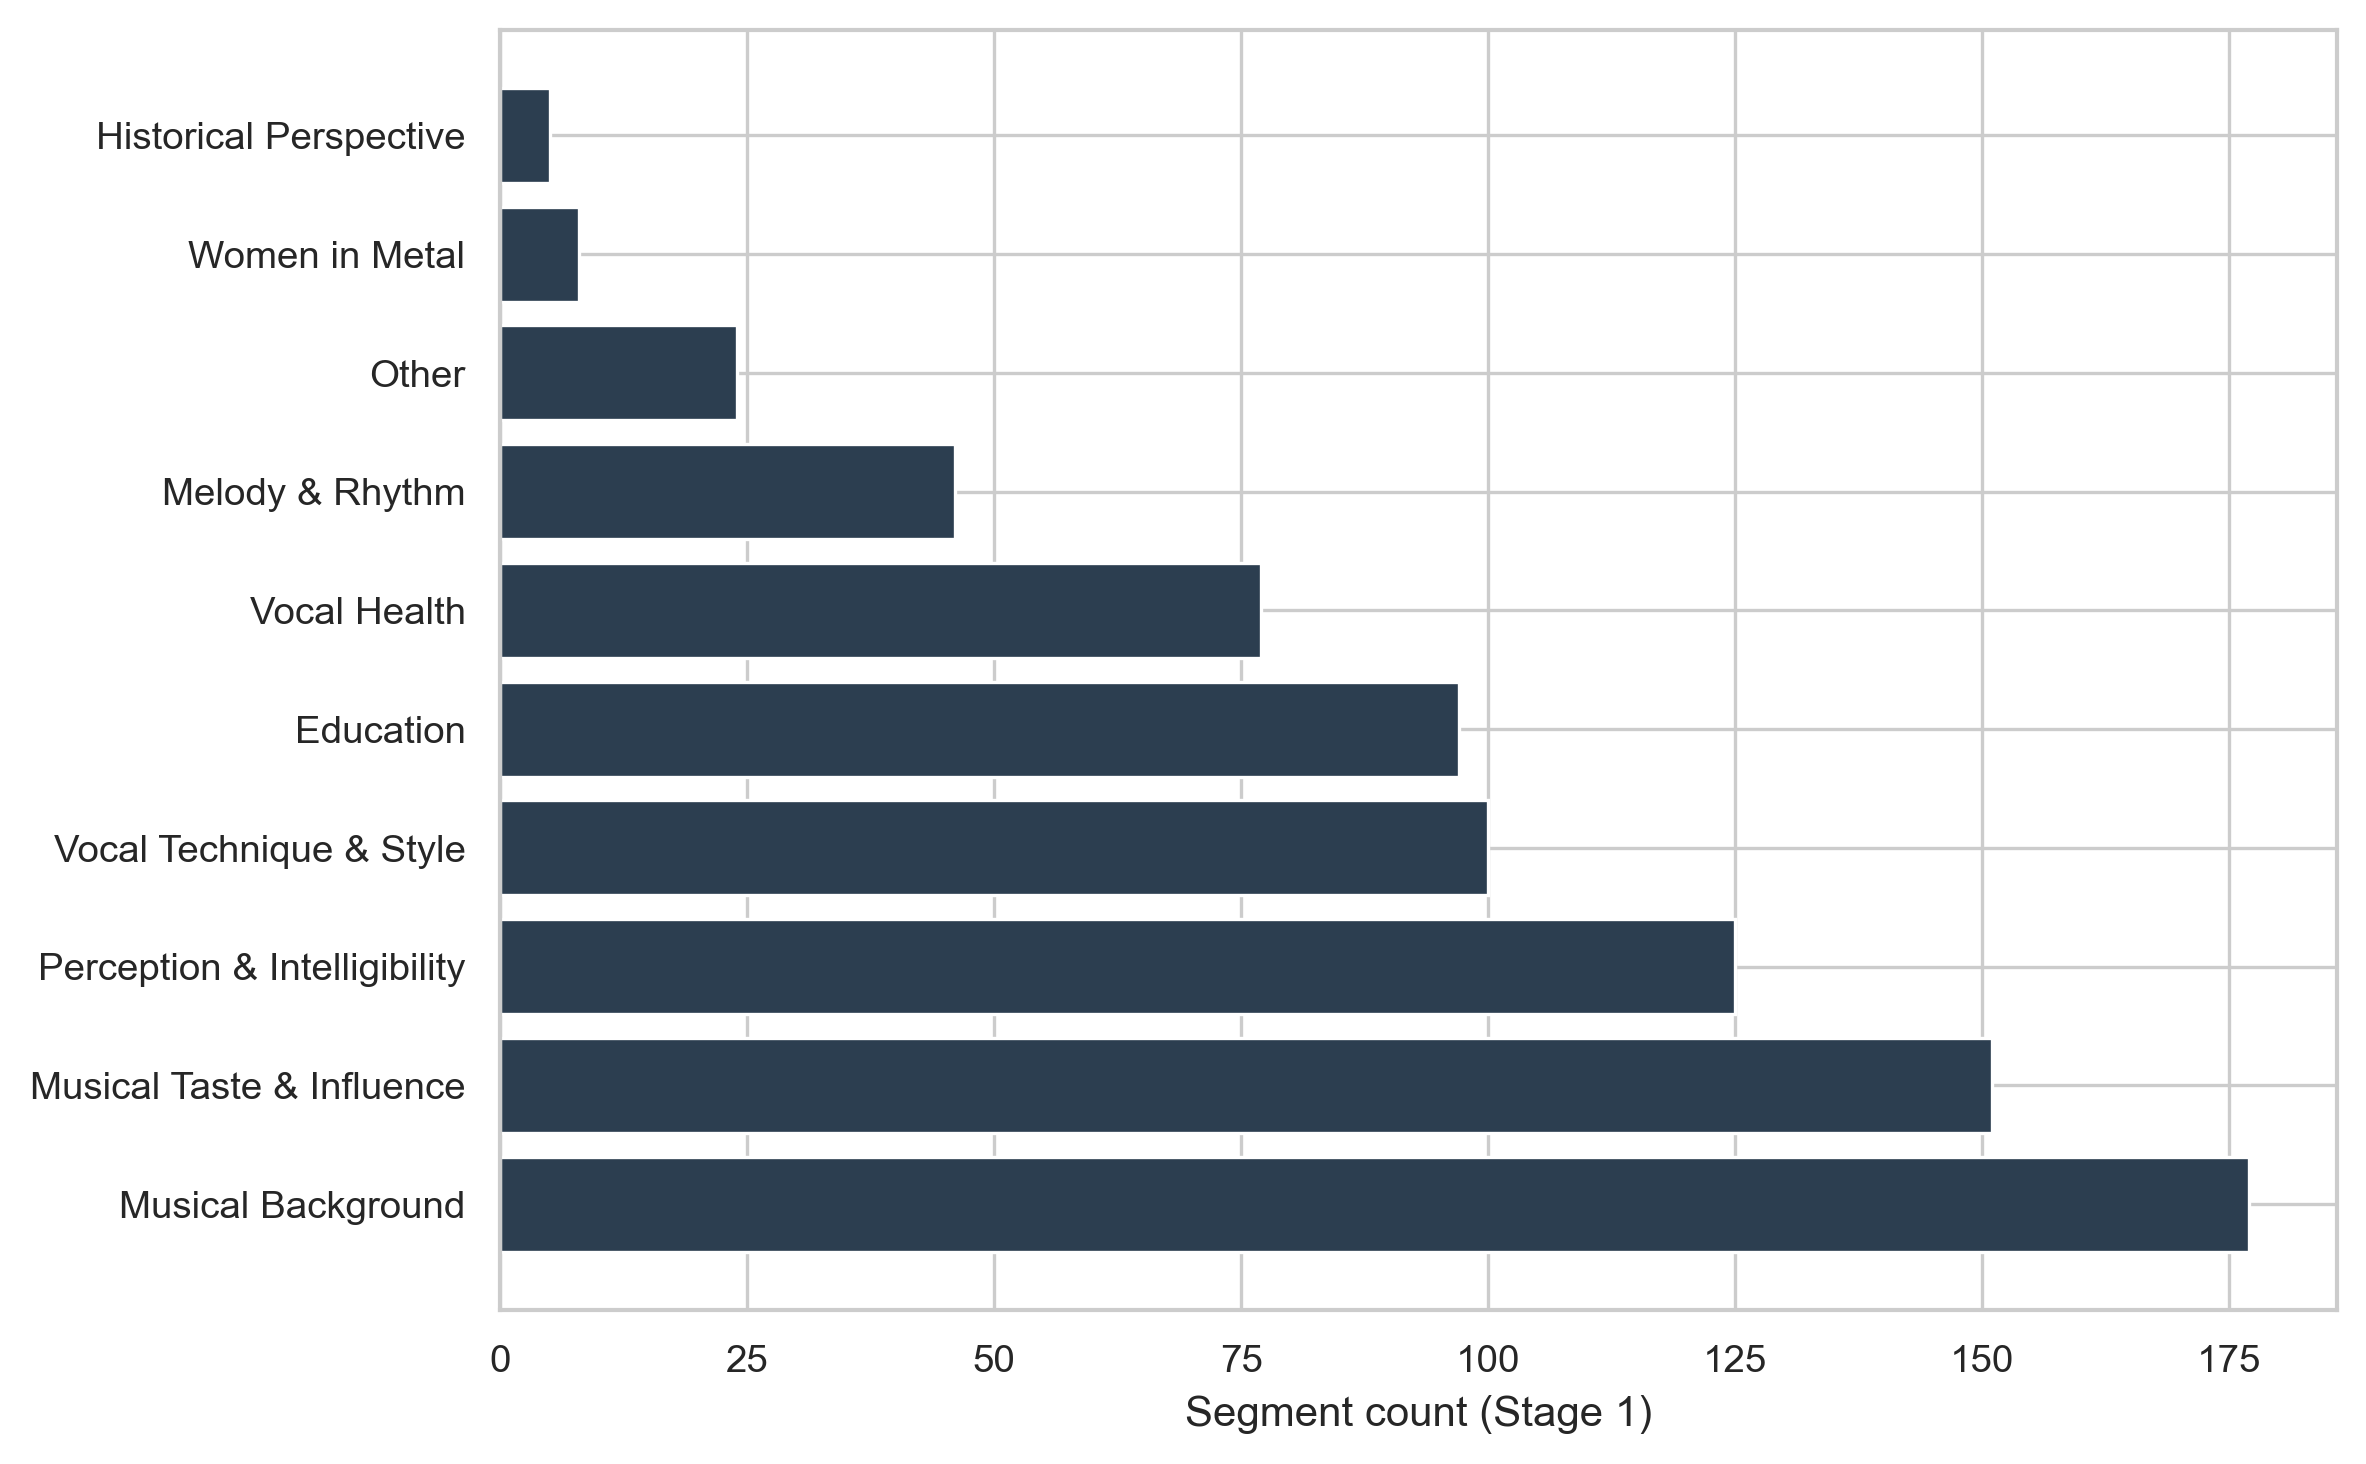
\includegraphics[width=0.92\linewidth]{stage1_themes_bar.png}
\caption{Stage 1 segment counts by thematic codebook category (\(N=810\) coded segments). Counts reflect how often each theme was applied at the segment level (multiple themes per answer possible across separate segments).}
\label{fig:stage1themesbar}
\end{figure}

\begin{figure}[ht]
\centering
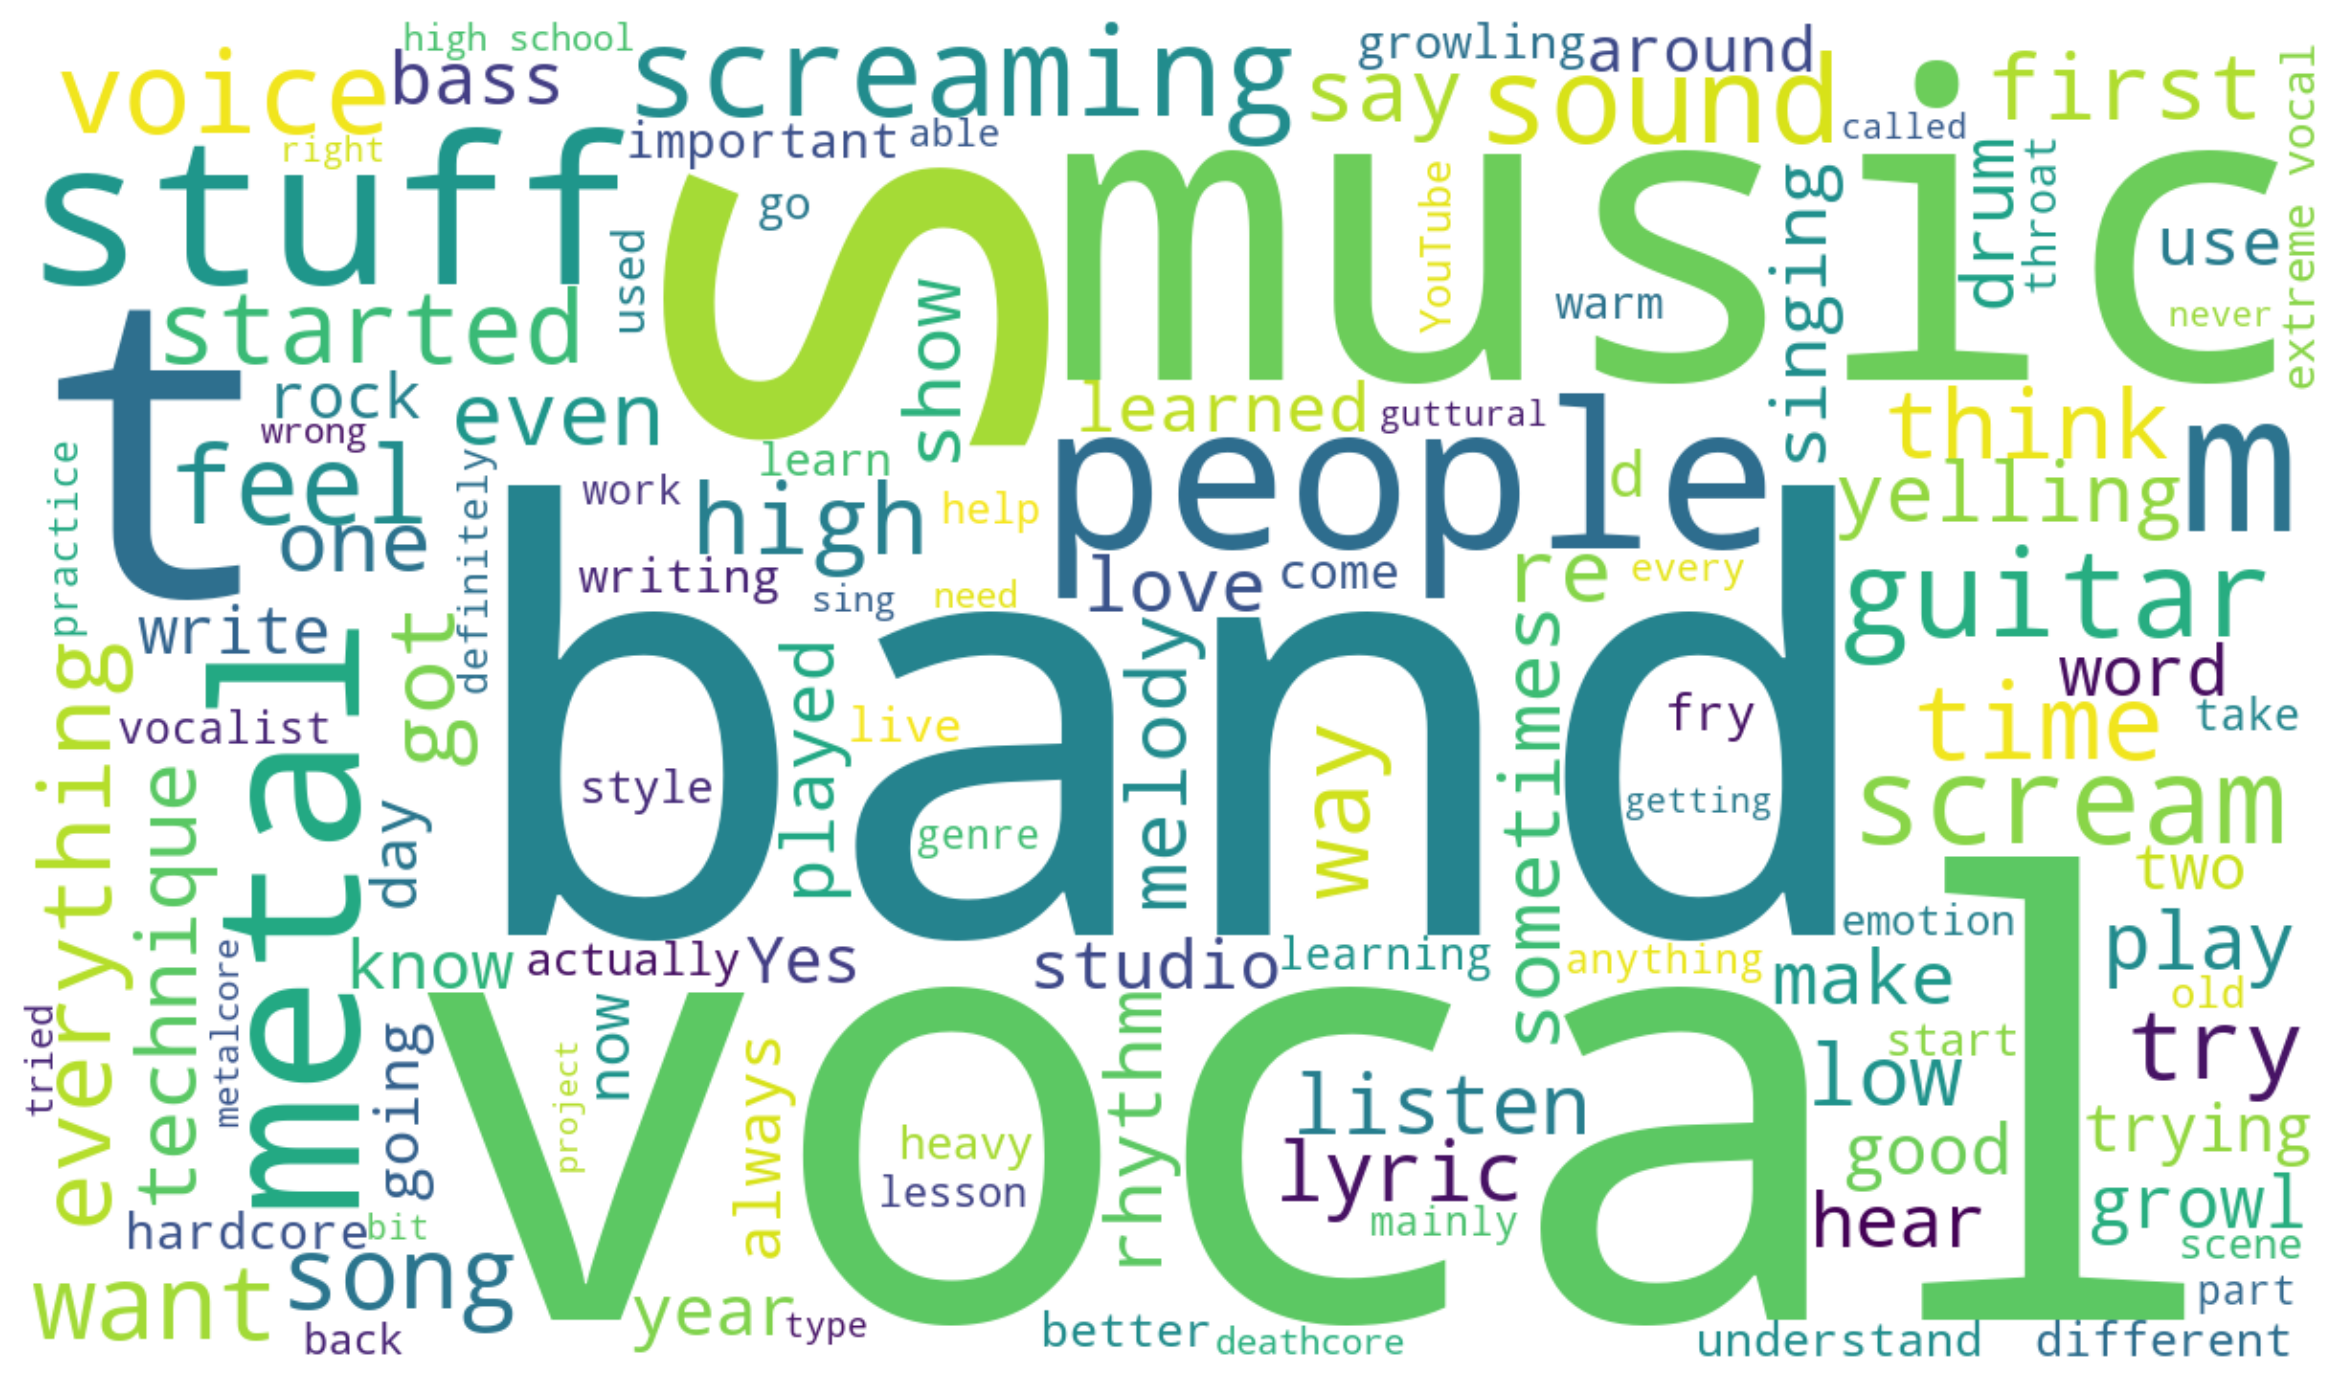
\includegraphics[width=0.95\linewidth]{wordcloud_stage1_all.png}
\caption{Illustrative word cloud for the full Stage 1 quotation corpus (English stopwords removed). The visualization highlights recurring lexical material but does not replace code-frequency analysis (see Limitations).}
\label{fig:wcloudall}
\end{figure}

\begin{figure}[ht]
\centering
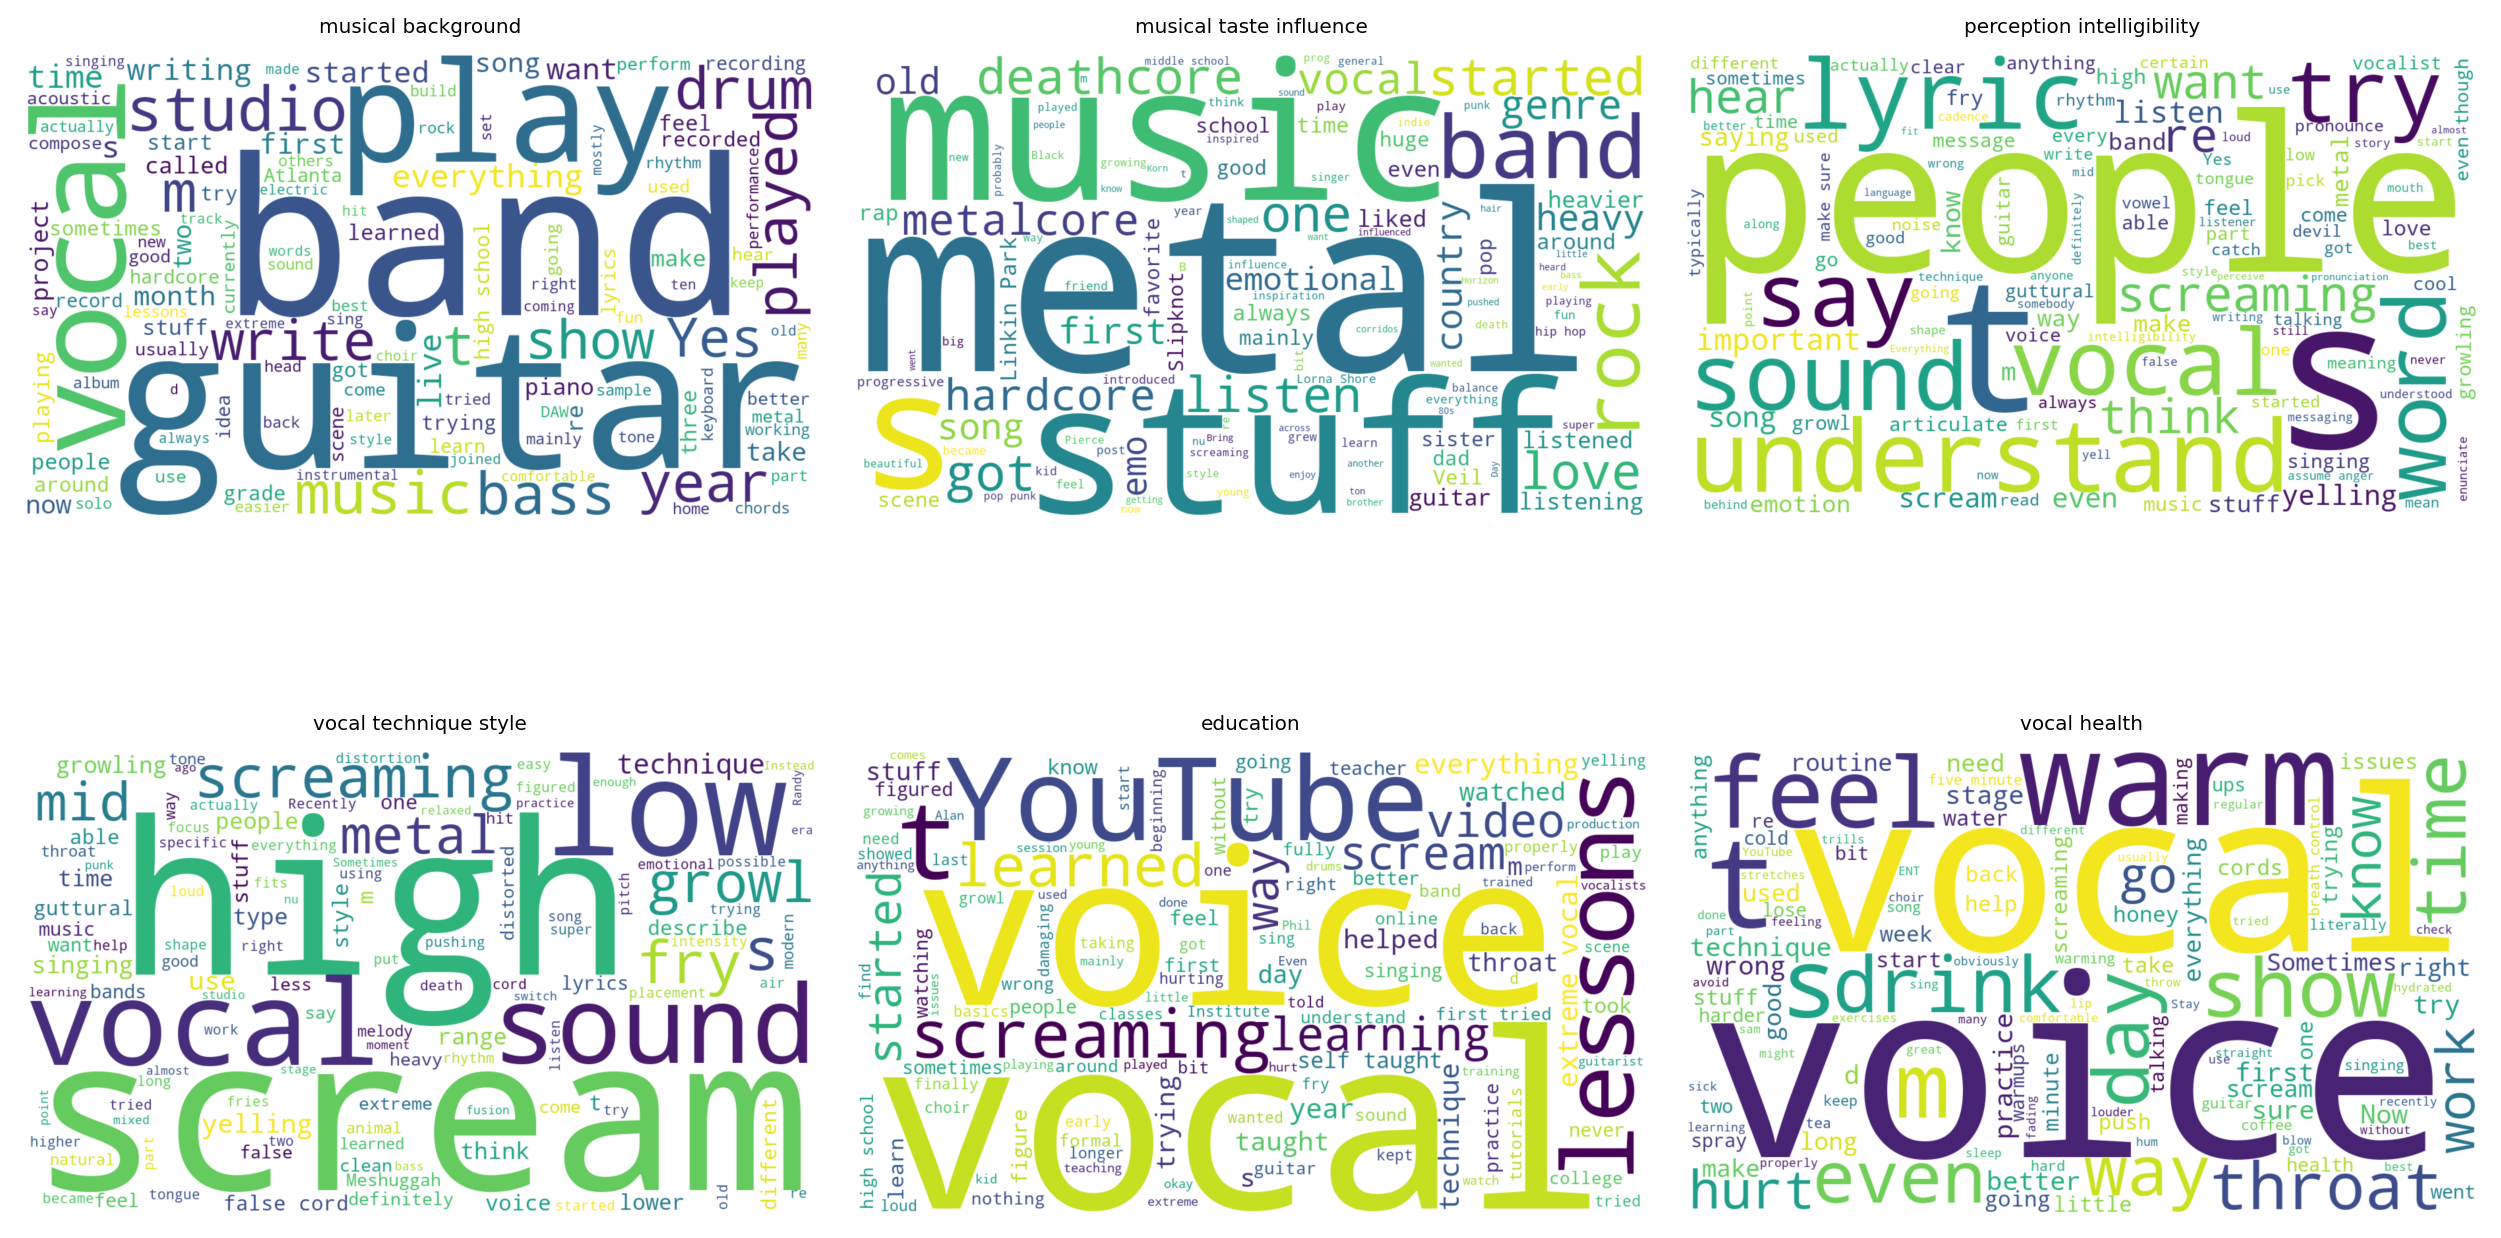
\includegraphics[width=\linewidth]{wordcloud_themes_montage.png}
\caption{Illustrative word clouds for the six largest Stage 1 themes (segment count \(\geq 40\)). Rare themes (e.g., Historical Perspective, Women in Metal) are summarized in text rather than plotted at small \(n\).}
\label{fig:wcloudmontage}
\end{figure}

Stage 1 is dominated by practical musician discourse (Table~\ref{tab:stage1themes}, Figure~\ref{fig:stage1themesbar}): background, influence histories, intelligibility concerns, and technique identity. Figures~\ref{fig:wcloudall}--\ref{fig:wcloudmontage} provide qualitative texture; interpretive claims below rely on coded themes and primary codes, not on word-cloud prominence. The distribution supports RQ1 and RQ2 by showing that participants do not isolate ``technique'' from broader contexts of scene history, pedagogy, and communication.

\subsubsection{Musical taste and influence}
Participants narrated gateway listening, subgenre loyalty, and cross-genre curiosity. Several described scene-adjacent social pathways into heavy music, while others emphasized solitary discovery through recordings and games. Representative excerpts include: ``Slipknot was a gateway band for metalcore and deathcore'' (Participant B); ``I listened to a ton of metal, hardcore, deathcore, metalcore\ldots\ I was raised in the scene'' (Participant C); ``Post hardcore---I love the balance of super singy stuff with the heavy'' (Participant E); ``My sister showed me\ldots\ My Chemical Romance and then Slipknot on the more extreme side'' (Participant F). The theme mixes canon bands (often named as shared reference points) with idiosyncratic non-metal taste that still shapes phrasing and dynamics.

\subsubsection{Musical background}
Interviewees reported heterogeneous musician profiles: multi-instrumentalists, lyric-focused writers, and vocal specialists. Many described DAW-centered writing workflows and demo-driven collaboration. Examples: ``I compose entire songs\ldots\ guitar is a tool to build off something catchy'' (Participant A); ``I tried learning guitar and drums\ldots\ I focused on singing and screaming at a very early age'' (Participant C); ``I've been in bands for almost 30 years\ldots\ from school orchestra to death metal projects'' (Participant K). These accounts situate vocal identity within band roles, recording habits, and touring or studio constraints.

\subsubsection{Education and learning pathways}
Formal classical or choral training co-occurred with self-teaching, peer coaching, and online pedagogy. Illustrative quotes: ``Completely self-taught in terms of instruments and vocals'' (Participant A); ``I was trained by my choir teacher\ldots\ for classical singing'' plus later ``Extreme Vocal Institute'' work (Participant C); ``YouTube and Reddit\ldots\ learning how to do it the safe way'' (Participant Q). The theme underscores iterative repair of technique after early misuse---a recurring narrative tied to health (below).

\subsubsection{Vocal technique and style}
Participants articulated register preferences, fry versus false-fold imagery, and stylistic blending across eras. Examples: ``When I want to enunciate a point, high fry is good'' (Participant B); ``I like to do vocal acrobatics\ldots\ use everything I have and not just one thing'' (Participant C); ``For high fries, definitely Randy Blythe\ldots\ for the lows, Levi Benton'' (Participant B); ``I pretty much only know fry scream'' (Participant R). These statements support H1: shared labels mask different default settings and artistic priorities.

\subsubsection{Vocal health and sustainability}
Narratives emphasized hydration, warm-ups, dietary triggers, pacing on tour, and clinical reassurance after symptoms. Examples: ``Number one: drink water\ldots\ if you wait until the show day it's too late'' (Participant B); ``I've had medical checks\ldots\ my vocal folds look great'' (Participant C); ``I don't drink soda\ldots\ room temp [water], because cold isn't very good for the vocal cords'' (Participant G); ``I would throw my voice out\ldots\ I was doing it very wrong'' (Participant F). The theme aligns with H2: protection behaviors are described as learned skills rather than innate traits.

\subsubsection{Perception and intelligibility}
Participants debated whether lyrics must be lexical-decodable for every listener, often linking intelligibility to rhythmic placement and songwriting intent. Examples: ``For me, people being able to understand what I'm doing is important'' (Participant C); ``Some people perceive yelling and screaming as negative---maybe from their upbringing'' (Participant B); ``Everything has to fit like a glove; otherwise we just got chaos'' (Participant A). These accounts frame harsh timbre as compatible with communicative intent when performers manage vowel shape and phrasing.

\subsubsection{Melody and rhythm}
Many participants rejected a melody-versus-chaos dichotomy, arguing that screamed lines still carry contour and temporal alignment with instruments. Examples: ``Melody or rhythm can help improve intelligibility---one hundred percent'' (Participant A); ``There's got to be a melody in there somewhere---you just have to find it'' (Participant B); ``A lot of djent songs\ldots\ the ostinato becomes the whole structure'' (Participant H). This complements the Stage~2 perceptual-class block by showing how performers reason about mid-level musical organization beneath timbral labels.

\subsubsection{Other (cross-cutting reflection)}
Segments coded as ``Other'' often foregrounded emotion regulation, artistic ethos, and motivation. Examples: ``It's not just about sounding cool---you've got to have something to say'' (Participant F); ``Metal is the most expressive and organized way to express yourself'' (Participant D); ``I want people to feel the emotion and the meaning'' (Participant J). These metacommentary segments contextualize technique choices as ethically and aesthetically motivated.

\subsubsection{Women in metal (scene positionality)}
Although \(n\) is small at the segment level, the theme carried consistent content about legitimacy and double standards. Examples: ``Women are discouraged from having a prominent, loud voice'' (Participant G); ``It's a very challenging scene to tap into and not be seen as a gimmick'' (Participant P). These excerpts connect vocal identity to reception norms rather than to acoustics alone.

\subsubsection{Historical perspective}
Participants occasionally situated their practice within band-era histories and local scenes. Examples: ``Kiss gave me appreciation for theatrical bands. Then I found Slipknot---Linkin Park kind of got me into screaming'' (Participant B); ``My hometown had a local band with two front guys---that was my first time seeing a hardcore band'' (Participant P). This theme provides timeline anchors that contextualize vocabulary acquisition.

\subsubsection{Top-mentioned bands and vocalists (coded influences)}
Table~\ref{tab:topbands} and Table~\ref{tab:topvox} summarize the most frequent explicit entries in \texttt{BAND\_INFLUENCE(\ldots)} and \texttt{VOCALIST\_INFLUENCE(\ldots)} tags across Stage~1 \texttt{Codes} fields. Counts are not exhaustive of every name spoken in interviews---only of segments where coders applied these tags. Some vocalist tags include non-metal artists when participants cited them as timbral or phrasing references.

\begin{table}[ht]
\centering
\caption{Top 15 band-level influence tags in Stage 1 \texttt{Codes} (frequency of tagged mentions).}
\label{tab:topbands}
\begin{tabular}{lr}
\toprule
Name & Count \\
\midrule
Slipknot & 5 \\
Linkin Park & 4 \\
Lorna Shore & 4 \\
My Chemical Romance & 3 \\
Chelsea Grin & 3 \\
Pierce the Veil & 3 \\
Korn & 2 \\
Lamb of God & 2 \\
The Devil Wears Prada & 2 \\
Black Veil Brides & 2 \\
Sepultura & 2 \\
Meshuggah & 2 \\
Green Day & 1 \\
M\"{o}tley Cr\"{u}e & 1 \\
Ratt & 1 \\
\bottomrule
\end{tabular}
\end{table}

\begin{table}[ht]
\centering
\caption{Top 15 vocalist-level influence tags in Stage 1 \texttt{Codes} (frequency of tagged mentions).}
\label{tab:topvox}
\begin{tabular}{lr}
\toprule
Name & Count \\
\midrule
Randy Blythe & 3 \\
Chester Bennington & 2 \\
Levi Benton & 2 \\
Mitch Lucker & 2 \\
Will Ramos & 2 \\
Landon Tewers & 2 \\
Alex Terrible & 2 \\
Brendon Urie & 1 \\
Davey Havoc & 1 \\
Ruki (the Gazette) & 1 \\
Bruno Mars & 1 \\
Charlie Puth & 1 \\
Vince Neil & 1 \\
Corey Taylor & 1 \\
Dickie Allen & 1 \\
\bottomrule
\end{tabular}
\end{table}

\subsection{Stage 2: Perceptual-Class Block}
\subsubsection{Q43 Agreement with Three-Class Framework}
\begin{table}[ht]
\centering
\caption{Agreement with three perceptual classes (Q43, \(N=45\)).}
\label{tab:q43}
\begin{tabular}{lrr}
\toprule
Response & \(n\) & \% \\
\midrule
Agree & 30 & 66.7 \\
Disagree & 11 & 24.4 \\
Uncertain & 4 & 8.9 \\
\bottomrule
\end{tabular}
\end{table}

Most respondents endorsed the framework (Table~\ref{tab:q43}), indicating practical intelligibility of the three-class model from the performer side.

\subsubsection{Q44 Technique-to-Class Mapping}
Q44 (\(N=38\)) showed a clear directional pattern with non-trivial overlap:
\begin{itemize}
    \item \textbf{Growl-leaning:} False Cord, low (32 growl-like), Guttural (30 growl-like).
    \item \textbf{Scream-leaning:} Fry, high (30 scream-like), Banshee scream (28 scream-like), Goblin scream (24 scream-like).
    \item \textbf{Bridge/overlap region:} False Cord, mid (18/21/22 across scream/growl/hybrid), Fry, low (14/21/13), Hardcore scream/Shout (14/5/27).
\end{itemize}

These data support RQ3 and H1: the classes are usable but gradient rather than mutually exclusive bins.

\begin{figure}[ht]
\centering
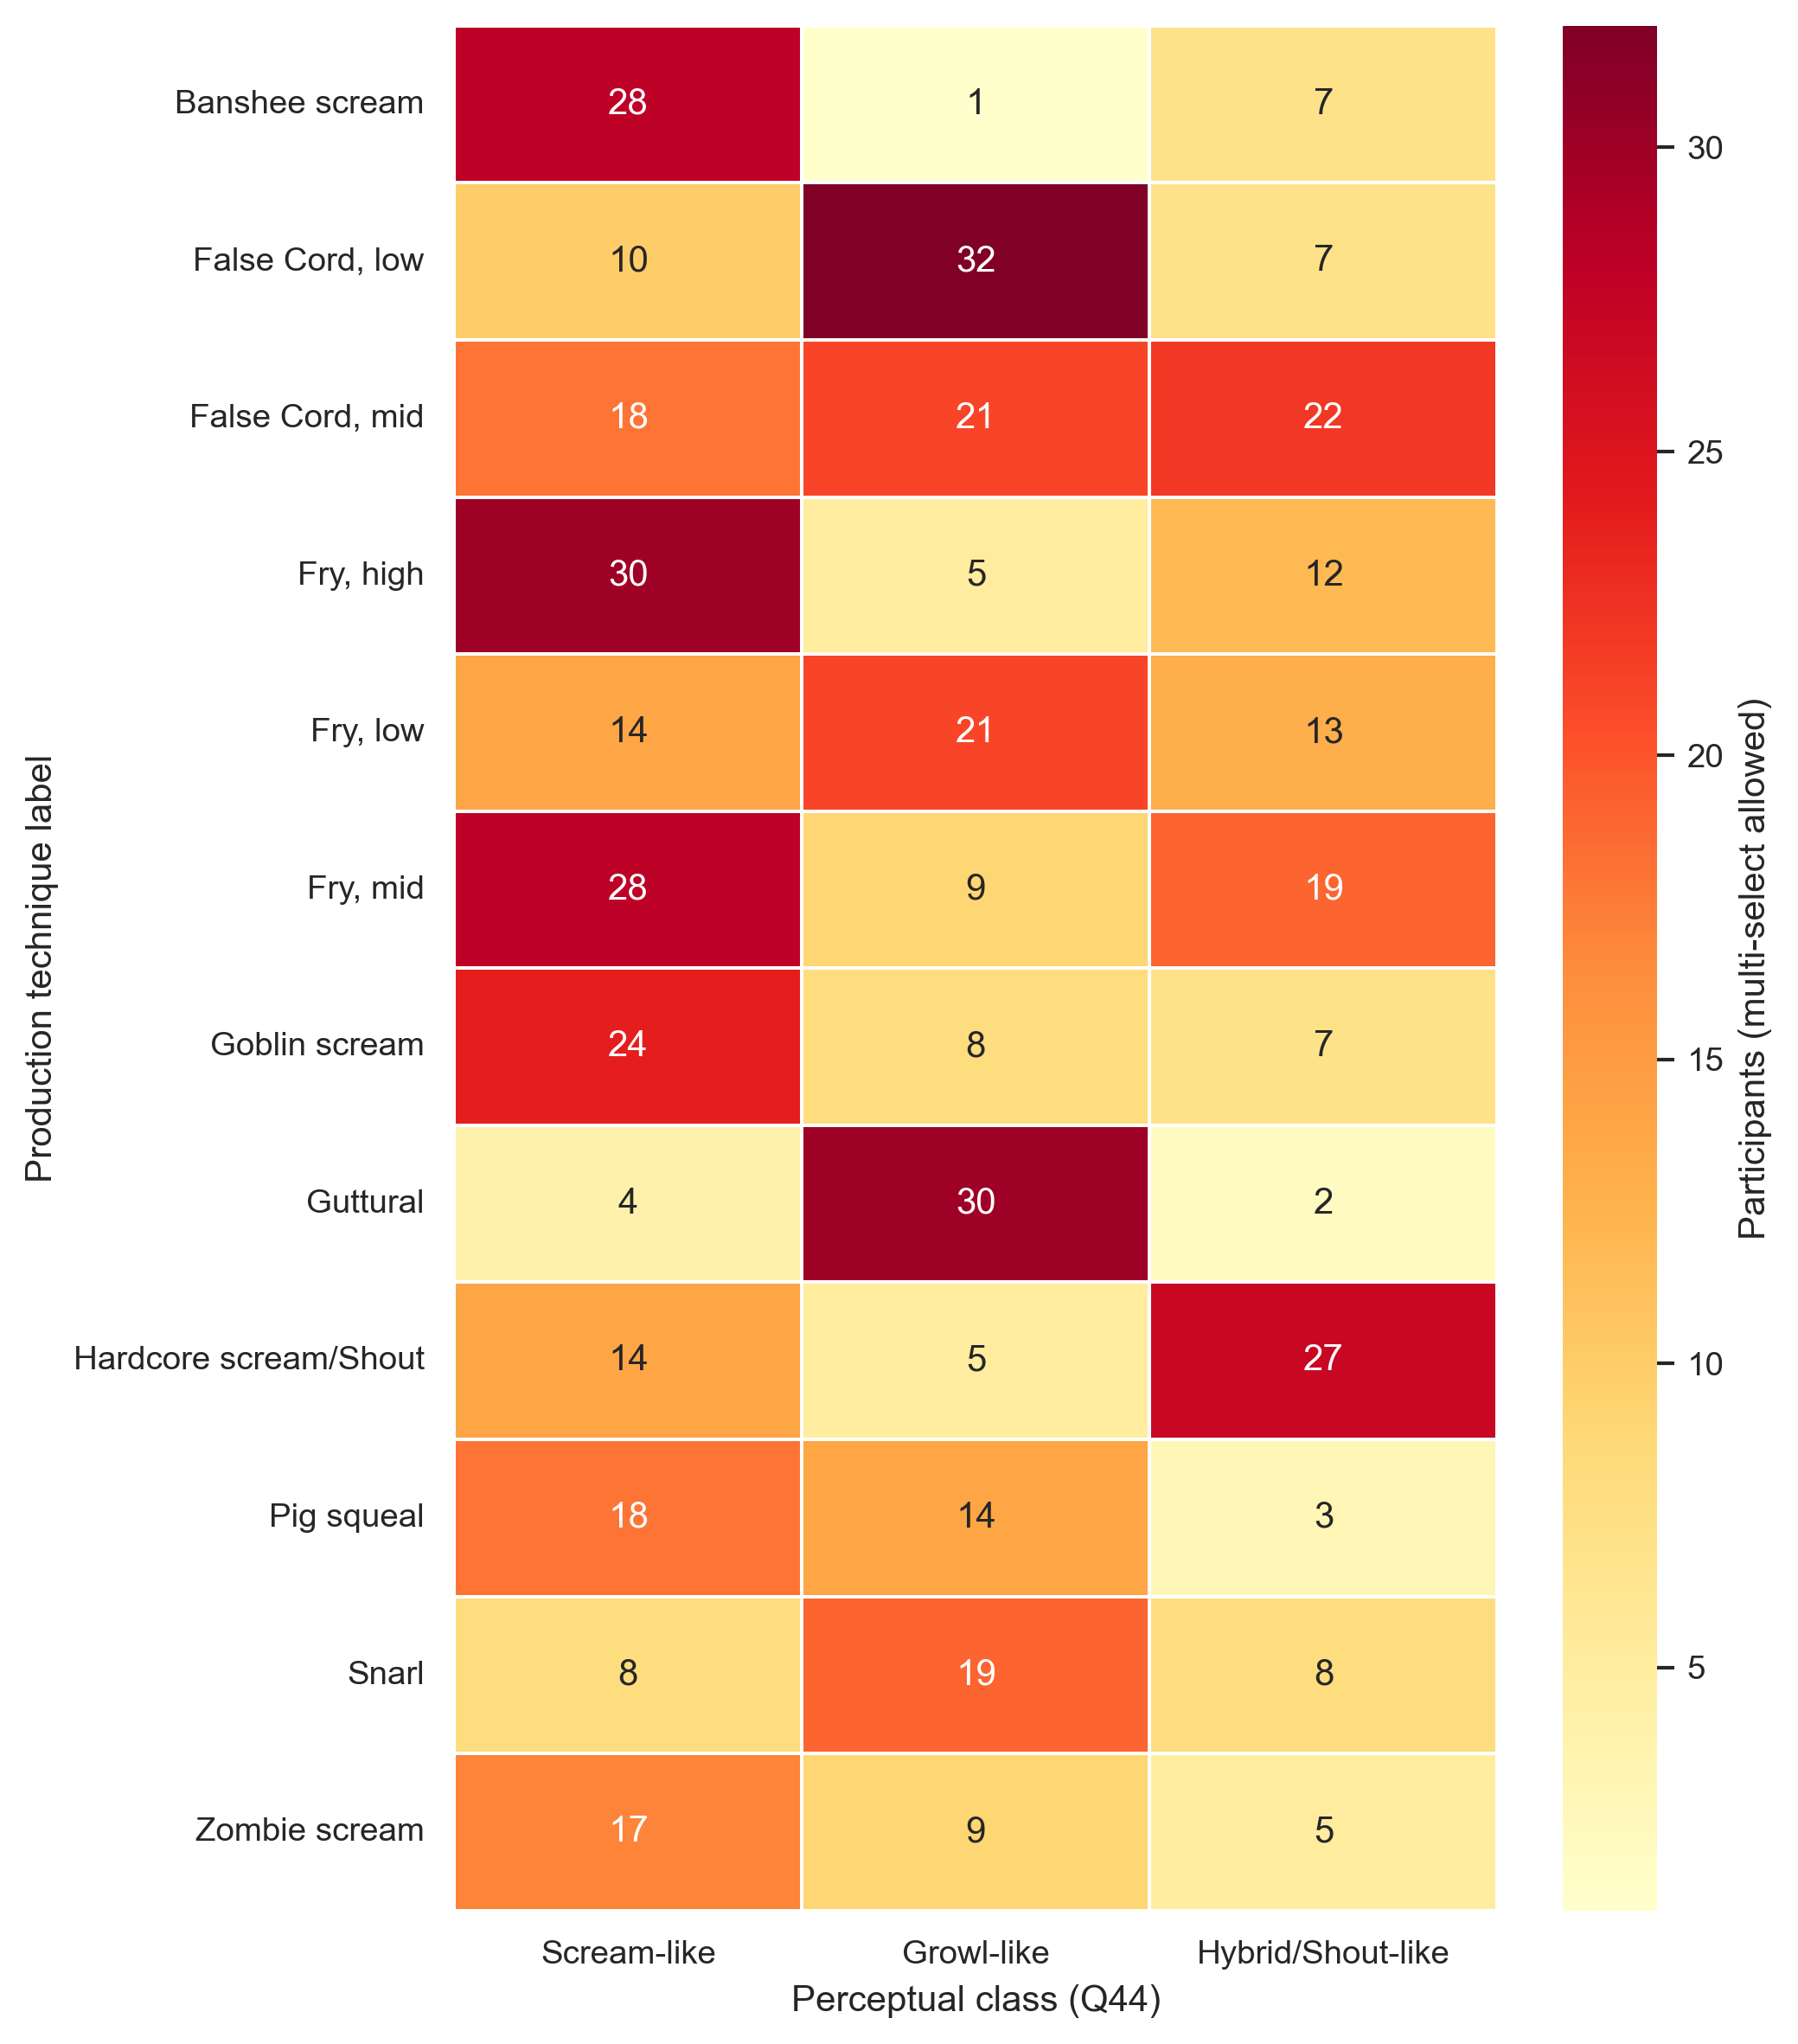
\includegraphics[width=\linewidth]{q44_heatmap.png}
\caption{Technique-to-class mapping (Q44). Cell values count participants who assigned the row technique to the column class (multiple selections allowed; \(N=38\) participants with at least one Q44 row answered). Darker cells indicate higher endorsement frequency.}
\label{fig:q44heat}
\end{figure}

Figure~\ref{fig:q44heat} mirrors Table~\ref{tab:stage2flow} coverage and visualizes the same counts exported in \texttt{q44\_mapping\_counts.csv}.

\subsubsection{Q45 Qualitative Associations}
In Q45 (\(N=33\) with all three fields completed), scream-like responses clustered around high-intensity affect (e.g., emotional, raw, aggressive), growl-like around heaviness/darkness imagery (e.g., demonic, brutal, animal metaphors), and hybrid/shout-like around mixed social-energy descriptors (e.g., gang-style, both, anger/sadness blends). The qualitative layer is consistent with Q44's overlap structure.

\subsubsection{Q46 Everyday Use of Class-Language}
\begin{table}[ht]
\centering
\caption{Self-reported use of perceptual classes in performance thinking (Q46, \(N=40\)).}
\label{tab:q46}
\begin{tabular}{lrr}
\toprule
Frequency & \(n\) & \% \\
\midrule
Regularly & 8 & 20.0 \\
Sometimes & 19 & 47.5 \\
Rarely/Never & 13 & 32.5 \\
\bottomrule
\end{tabular}
\end{table}

Table~\ref{tab:q46} suggests that production-language still dominates routine self-monitoring, while perceptual classes function as a secondary but available framework.

\subsection{What Stage 2 Adds Beyond Stage 1}
Stage 2 extends the analytical frame in two ways. First, it operationalizes class-level judgments directly (Q43--Q46), allowing explicit estimation of agreement, overlap, and usage frequency. Second, it broadens topical coverage through survey open-text fields that capture additional performer reflection on communication goals, historical positioning, and social interpretation in a structured response environment. In this sense, Stage 1 and Stage 2 are complementary: interviews preserve narrative nuance, while survey structure enables reproducible class-mapping summaries.

\paragraph{Illustrative Stage 2 open-text excerpts (de-identified).}
Survey respondents sometimes articulated production logic in fine detail; for example, one wrote that fry and hardcore screams can share a ``base technique'' differentiated by tension and projection, while another described mapping tunnel screams, gutturals, and whistle-like highs as distinct tools for different sections. A third emphasized breath support and sustainable loudness across a set rather than isolated ``trick'' techniques. These excerpts align with Stage~1's gradient framing: performers reason with inventories of gestures, then situate them in musical and pragmatic context.

\subsection{Cross-Stage Synthesis}
Taken together, Stage 1 and Stage 2 show a coherent pattern:
\begin{enumerate}
    \item performer discourse is production-rich and context-heavy (training, health, performance setting);
    \item broad perceptual grouping is largely interpretable and practically deployable when explicitly prompted;
    \item overlap is a structural feature of the data, especially in mid-register and mixed-intent techniques.
\end{enumerate}

This supports H3: Stage 2 broadens thematic and interpretive coverage without replacing Stage 1's production-centered narrative core.

\section{Discussion}
The principal contribution is methodological and conceptual: a staged design can preserve the granularity of performer language while testing a compact perceptual scaffold that is usable in broader communication. For voice-science and pedagogy audiences, this matters because teaching and assessment frequently move between concrete motor cues and listener-facing descriptors.

The data do not support a rigid taxonomy in which each technique maps cleanly to a single class. Instead, they support a \emph{gradient model} with stable poles and porous boundaries. This is especially clear for mid-register and hybridized techniques, where context, intensity, and stylistic intent appear to shift perceived class-membership. This interpretation is consistent with listener-side findings that categories are detectable but not perfectly discrete, and with acoustically heterogeneous technique inventories in recent dataset work \parencite{Pinto2023VocalEffects,Tailleur2021AcousticSpace,tailleur2024emvddatasetdatasetextreme,Tailleur2024EMVD}.

The health discourse in Stage 1 is also noteworthy. Participants repeatedly framed sustainability as an active practice (hydration timing, warm-up design, pacing, and load management), reinforcing current evidence that extreme effects are not inherently pathological when executed with control \parencite{Aaen2024ExtremeVocalEffects,Guzman2018MetalSinging,blomgren1998vocalfry}. At the same time, the interview material indicates that performers often learn this ``control'' through iterative experimentation before formalizing terminology, which helps explain why production-language remains central in Q46 despite broad comprehension of class labels.

Finally, the social layer (including gendered scene experience) indicates that technique identity is not purely acoustic or physiological; it is also mediated by performance culture, audience expectation, and legitimacy narratives \parencite{Herbst2017VoiceOfAnarchy,Wallmark2018SoundOfEvil,Ribaldini2019Terminology}. This has practical implications for pedagogy and applied voice communication: terminologies that are technically precise but culturally tone-deaf may fail to translate into performer adoption.

From a methods perspective, the staged design also clarifies claim strength. We treat interview themes and survey mappings as convergent descriptive evidence rather than inferential causal proof. That stance is intentional and aligns with the goal of producing a robust performer-centered frame that can support future inferential and longitudinal work.

\section{Limitations}
First, Stage 2 is a convenience sample with uneven item completion, and item-specific \(N\) varies substantially across Q43--Q46 and broader open-text blocks. Second, Stage 1 contains a documented assisted completion subset (76 rows), which improves coverage but should be interpreted as reproducible interim coding rather than final adjudicated consensus coding. Third, the manuscript focuses on descriptive interpretation rather than inferential testing; future work should report formal uncertainty and reliability metrics for both coding and class-assignment structures.

Additional constraints include possible self-selection effects (participants already engaged with extreme-vocal discourse), language/context effects in open-text responses, and unavoidable mismatch between segment-level interview counts and respondent-level survey counts in cross-stage summaries. Word clouds are illustrative: token prominence depends on stopword settings and preprocessing and should not be read as a substitute for the codebook-driven theme counts in Table~\ref{tab:stage1themes}.

\section{Conclusion}
This study presents a reproducible two-stage performer-centered analysis of extreme metal vocal practice. Stage 1 interview data demonstrate that technique, health, intelligibility, and musical identity are deeply interwoven in everyday reasoning. Stage 2 survey data show that a three-class perceptual scaffold is meaningful for most respondents, but technique-to-class mapping remains overlapping and gradient.

Taken together, the findings support a practical taxonomy that is useful for communication across performer, pedagogical, and research contexts without overstating categorical rigidity. Future work should prioritize multi-coder reliability expansion, broader sampling across scenes, and tighter integration with acoustic feature-space modeling so that performer language, perceptual structure, and measurable signal properties can be linked more directly.

\section*{Funding}
No external funding is declared for this manuscript draft.

\section*{Data Availability}
Public artifacts include de-identified processed datasets and reproducible scripts. Raw participant-linked materials remain restricted for ethical and privacy reasons.

\section*{Declaration of Competing Interest}
The authors declare no known competing financial interests or personal relationships that could have appeared to influence the work reported in this paper.

\section*{Appendix A. Consolidated Stage 1 interview prompts (reference protocol)}
\label{app:stage1}

Across the 18 sessions, numbering and exact wording varied with pilot revisions; the following consolidated list reflects the most complete linear protocol used (e.g., Participant C) plus common follow-ups seen in other transcripts. Not every participant received every probe in identical order.

\paragraph{Musical taste and listening.}
How did you get into music? How did you get into metal, and what inspired you? Which metal genres and subgenres do you listen to, and why? Which other genres do you listen to besides metal?

\paragraph{Musical background and activity.}
Do you play instruments? Do you compose music? Do you have formal musical education? Are you currently in a band (name, tenure, role)? Have you been in other bands? How often do you perform live? How often do you record (studio or home studio)? Do you notice differences between live and studio vocal approach? How long have you been active as a singer or extreme vocalist?

\paragraph{Learning and technique.}
How did you learn extreme vocal techniques? Have you taken vocal lessons; did they cover extreme techniques? Do you follow warm-ups or routines? What strategies protect your voice from strain? Have you experienced vocal health problems related to extreme singing? How would you describe your vocal style? Which bands or vocalists influenced you? Which techniques do you use most frequently?

\paragraph{Perception, intelligibility, melody, and rhythm.}
Is intelligibility an important goal? How do you make lyrics intelligible with extreme techniques? Why might non-metal listeners find extreme vocals hard to understand? Why might some people dislike metal? How do you think about pitch, melody, and rhythm in extreme vocals? Can extreme vocals convey melody? Can they convey rhythm?

\paragraph{Additional probes used in some sessions (examples).}
Follow-up prompts such as subgenre detail, gateway artists, non-metal taste, gutturals and melody, combined melody/rhythm blocks, women in metal, historical change in bands, and open reflection on emotion and identity appeared when the conversation required clarification or depth.

\section*{Appendix B. Stage 2 (Qualtrics) items not represented in Appendix A}
\label{app:stage2}

The online survey added structured demographics, screening, inventories, and a dedicated perceptual-class block. Full consent language was shown per jurisdiction in Qualtrics; below are substantive research items only. Items Q47--Q53 in the survey overlap thematically with intelligibility/melody/rhythm prompts in Stage 1 and are omitted here to avoid duplication; they were retained in the dataset for cross-format comparison.

\paragraph{Ethics and screening.}
Origin-based consent routing; general participation consent; jurisdiction-specific consent where applicable; screening: ``Are you an active or former metal vocalist?''

\paragraph{Demographics.}
Age; gender (including free-text when ``other''); native language(s) learned at home; country of residence (optional).

\paragraph{Metal and non-metal taste (structured).}
Which metal genres and subgenres do you listen to regularly (multi-select, including other-specify)? Why do you like these genres? Which non-metal genres do you listen to (multi-select, including other-specify)? Why do you like those genres?

\paragraph{Musicianship and creative practice.}
Self-reported musicianship level; instruments and years of experience; whether you compose; description of composing workflow and tools; formal musical education (yes/no) and narrative description of training.

\paragraph{Band history and performance context.}
Current band membership and roles; tenure; past bands (names, roles, years); live performance frequency; recording experience in professional and/or home studios (narrative).

\paragraph{Vocal career, training, and health (survey form).}
Years active as extreme vocalist; formal vocal lessons (yes/no) and descriptions of private lessons, online learning, and peer learning; how extreme techniques were learned (structured choices plus other-specify); vocal exercise and health routines; strategies to prevent strain; history of vocal health problems (narrative); self-description of vocal style.

\paragraph{Influence and technique use (open and checklist).}
Free-text: which vocalists or bands influenced your style. Checklist: which labeled techniques you use most frequently (with other-specify); additional techniques in free text; differences between live and studio approach.

\paragraph{Perceptual-class focal block (Q43--Q46).}
Agreement with grouping harsh vocals into scream-like, growl-like, and hybrid/yell-like classes; optional comment on revising the system; matrix mapping each listed production technique to one or more classes (or not sure); open associations (emotions, imagery) for each class; self-reported frequency of thinking in those class terms while singing.

\paragraph{Historical and meta items (examples).}
Earliest recalled examples of growl, scream, and hybrid/yell vocals in metal or broader music history; whether animal comparisons help describe extreme vocals; open comments on classification and research; additional critiques or suggestions.


\printbibliography
\end{document}

